\documentclass[../main.tex]{subfiles}
\begin{document}
	\begin{examples}\
		\begin{mylist}
		\item 
		$f: [a, 2\pi] \rightarrow \R(\mathbb C)\\
		f$ -- $2\pi$ период.\\
		$(f, g) = \mathlarger{\int}_0^{2\pi} f(x) \vec g (x) dx$
		\begin{mylist}
			\item 
			$\R\\
			\underset{\text{попарно-ортог.}}{1, \sin x, \cos x, \sin 2x, \cos 2x, \ldots} \; \; \; \; 
			\underset{\text{вещ.}}{([0, 2\pi])}\n
			(\cos k x, \sin m x) = \mathlarger{\int}_0^{2\pi} \cos k x \sin m x dx = \frac{1}{2} \mathlarger{\int}_0^{2\pi}
			(\sin(m+k) x + \sin (m-kx))dx = 0\n
			(\sin k x, \sin mx) = \mathlarger{\int}_0^{2\pi} \sin kx \sin m x dx = -\frac{1}{2} \mathlarger{\int}_0^{2\pi}
			(\cos(m+k) x - \cos(m-kx))dx = 0$\n
			И т.д.\\
			$\underset{k\neq 0 \; = \|\sin k x\|}{\|\cos kx\|} = \sqrt{(\cos kx, \cos kx)} = (\mathlarger{\int}_0^{2\pi} \cos^2 kx dx)^\frac{1}{2} = 
			(\mathlarger{\int}_0^{2\pi} \frac{1+\cos 2kx}{2} dx)^\frac{1}{2} = \sqrt{\pi}\n
			\|1\| = \sqrt{(1, 1)} = \sqrt{\mathlarger{\int}_0^{2\pi} 1 dx} = \sqrt{2\pi}$
			\item 
			$\mathbb C \; \; \underset{\text{попарно-ортог.}}{\{e^{ikx}\}_{k=-\infty}^{+\infty}} \; \; \; \; (e^{ikx}, e^{imx}) = \mathlarger{\int}_0^{2\pi} e^{ikx} e^{-imx} dx = \mathlarger{\int}_0^{2\pi} e^{i(k-m)x} dx = \n
			\underset{k\neq m}{=} \frac{1}{i(k-m)} e^{i(k-m)x}\bigg|^{2\pi}_0 = 0\n
			\underset{k=m}{=} \|e^{ikx}\|^2 = \mathlarger{\int}_0^{2\pi}1dx = 2\pi\n
			\|e^{ikx}\| = \sqrt{2\pi}$
		\end{mylist}
		\item 
		$P_n$ многочлены $deg\leq n \subset L^2([-1, 1])\n
		\forall p, q \in P_n \; \; \; (p, q) = \mathlarger{\int}_{-1}^1 p(x) q(x) dx \; \; \; \; \; \; P_n = span\underset{\text{канон. базис}}{1, x, x^2, \ldots, x^n}\n
		\underset{k\neq m}{(x^k, x^m)} = \mathlarger{\int}_{-1}^1 x^{k+m} dx \left\{\\
			\begin{matrix}
				\neq 0 & k+m \text{ -- четн}\\
				= 0 & k+m \text{ -- нечетн.}
			\end{matrix}\right.\n
		1, x, x^2, \ldots, x^n \; \; \text{Ортогонализуем Г-Ш}\n
		\begin{matrix}
			b_1 = 1\\
			b_2 = a_2 - c_1b_1
		\end{matrix} \; \; c_1 = \mathlarger{\frac{(a_2. b_1)}{(b_1, b_1)}} \; \; \; 
		\begin{matrix}
			(b_1, b_1) = \mathlarger{\int}_{-1}^1 1\cdot 1 dx = 2\n
			(a_2, b_1) = \mathlarger{\int}_{-1}^1 x\cdot 1 dx = 0
		\end{matrix}\n
		b_3 = a_3 - \tilde{c_1} b_1 - \tilde{c_2} b_2 \; \; \; 
		\begin{matrix}
			\tilde{c_1} = \mathlarger{\frac{(a_3, b_1)}{(b_1, b_1)}}\\\\
			\tilde{c_2} = \mathlarger{\frac{(a_3, b_2)}{(b_2, b_2)}}
		\end{matrix}
		\; \; \; \; \begin{matrix}
			(b_1, b_2) = \mathlarger{\int}_{-1}^1 x^2 dx = 2\mathlarger{\int}_0^1 x^2 dx = \frac{2}{3}\n
			(a_3, b_1) = \mathlarger{\int}_{-1}^1 x^2 \cdot 1 dx = \frac{2}{3}\n
			(a_3, b_2) = \mathlarger{\int}_{-1}^1 x^2 \cdot x^ dx = 0
		\end{matrix}\n
		b_3 = x^2 - \frac{2}{3} \cdot \frac{1}{2} \cdot 1 = x^2 - \frac{1}{3}\n
		b_4 = x^3 - \frac{3}{5} x$\n
		$P_n = span(1, x, \ldots, x^n) \underset{\text{Г-Ш}}{\leadsto} l_0(x) = 1 \; \; \underset{\text{попарно-ортог.}}{l_1 (x) = x \; \; \; l_2(x) = x^2-\frac{1}{3}} \; \; \; 
		\underset{\text{\large{Полиномы Лежандра}}}{l_3(x) = x^3 - \frac{3}{5} x \ldots}$\n
		$\boxed{\text{н.у.о.} \rightarrow \; \; l_k(x) = \lambda_k((x^2-1)^k)^{(k)} \text{  Общая ормула полиномов Лежандра с точностью до const}}$
		\begin{proof}
			$q_k(x) = ((x^2 - 1)^k)^{(k)} \; \;  \; deg \ q_k = k\n
			\forall m = 0, \ldots, k-1 \; \; \; \; (q_k, x^m) = \mathlarger{\int}_{-1}^1 ((x^2 - 1)^k)^{(k)} x^m dx =
			\mathlarger{\int}_{-1}^1 x^m d((x^2 - 1)^k)^{(k-1)} \n
			\boxed{f' dx = df}\n
			= x^m (\underset{\mathlarger{\underset{\text{2 корня: } \pm 1 \text{ кр-ти } k}{=(x-1)^k (x+1)^k}}}{(x^2 - 1)^k})^{(k-1)} \bigg |_{-1}^1 - \mathlarger{\int}_{-1}^1 ((x^2 - 1)^k)^{(k-1)} \underbrace{dx^m}_{m x^{m-1} dx} = -m \mathlarger{\int}_{-1}^1 x^{m-1} d((x^2 - 1)^k)^{(k-2)} = \ldots\n
			= \pm m! \mathlarger{\int}_{-1}^1 ((x^2-1)^k)^{(k-m)} dx = \pm m! ((x^2 - 1)^k)^{(k-m-1)} \bigg |_{-1}^1 = 0\n
			L = span(1, \ldots, x^{k-1}) \n
			q_k \perp L\n
			deg\ q_k = k \; \; \; \; span(q_0, q_1, \ldots, q_k) = span(1, x, \ldots, x^k)$\n
			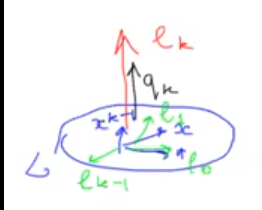
\includegraphics[width=150px]{pic03}\n
			$\Rightarrow \lambda_k q_k = l_k (x)$
		\end{proof}
		$q_k(1) = (\underset{= (x-1)^k (x+1)^k}{(x^2 - 1)^k})^{(k)}\bigg |_{x=1} = \sum\limits_{m=0}^k C^m_k ((x+1)^k)^{(m)} (\underset{= 0 \; \; m\neq 0}{(x-1)^k})^{(k-m)}\bigg |_{x=1} = \n
		\text{Применили формулу Лейбница для взятия производной}\n
		= (x+1)^k ((x-1)^k)^{(k)}\bigg |_{x=1} = 2^k k!\n
		\boxed{
			\begin{matrix}
			l_k(x) = \mathlarger{\frac{1}{2^k k!}} ((x^2 - 1)^k)^{(k)}\n
			l_k (1) = 1
			\end{matrix}
		}$\n
		\textbf{Формула Родрига} для полиномов Лежандра\n
		\n
		$\|l_k\|^2 = \mathlarger{\int}_{-1}^1 \underbrace{(\frac{1}{2^k k!})^2}_A ((x^2 - 1)^k)^{(k)} \underbrace{((x^2 - 1)^k)^{(k)} dx}_{d((x^2 - 1)^k)^{(k-1)}} = \n
		A ((x^2 - 1)^k)^{(k)} ((x^2 - 1)^k)^{(k-1)} \bigg |_{-1}^1 - A\mathlarger{\int}_{-1}^1 ((x^2-1)^k)^{(k-1)} \underbrace{d((x^2-1)^k)^{(k)}}_{((x^2-1)^k)^{(k+1)} dx} = \n
		= (-1)^k A \mathlarger{\int}_{-1}^1 \underbrace{((x^2-1)^k)^{(2k)}}_{(2k)!} (x^2 - 1)^k dx = (-1)^k A (2k)! \ \ 2 \mathlarger{\int}_0^1 \underset{= (-1)^k (1-x^2)^k}{(x^2-1)^k} dx =\n
		\underset{\begin{matrix}
			x = \sin t\\
			dx = \cos t dt
			\end{matrix}}{=} \frac{(2k)!}{2^{2k-1} (k!)^2} \mathlarger{\int}_0^{\frac{\pi}{2}} \cos^{2k+1} t dt = \n
		\slide{300px}\mathlarger{\int}_0^{\frac{\pi}{2}} \cos^{2k+1} t dt = \frac{(2k)!!}{(2k+1)!!} = \frac{2^k k!}{(2k+1)!!} \n
		= \mathlarger{
			\frac{(2k)! 2^k  \cdot k!}{2^{2k-1} (k!)^2 (2k+1)!!} = \frac{(2k)!  2}{\underbrace{\underbrace{2^k k!}_{(2k)!!} (2k+1)!!}_{(2k+1)!}} = \frac{2}{2k+1}
		}\n
		\|l_k\| = \sqrt{\mathlarger{\frac{2}{2k+1}}}\n
		\boxed{\mathlarger{\sqrt{\frac{2k+1}{2}}\frac{1}{k! 2^k} ((x^2-1)^k)^{(k)}} \text{   Нормиров. система полиномов Лежандра}}$\\
		\item 
		$L^2([-1, 1], \frac{dx}{\sqrt{1-x^2}}$ Скалярное произведение с весом\n
		$(f, g) = \bint_{-1}^1 f\cdot g \frac{dx}{\sqrt{1-x^2}}$\n
		\underline{Многочлены Чебышёва} $\; \; \; \; T_k(x) = \underset{\text{ортогон. система}}{\cos(k\cdot \arccos x) \; k = 0, 1, 2 \ldots}\n
		T_0 (x) = 1 \; \; T_1(x) = x \; \; \; T_2 = 2x^2 - 1\n
		\underset{k\neq 0 }{(T_k, T_m) = 0}\n
		deg T_k = k$
		\item 
		$L^2(\R, e^{-x^2} dx)$\n
		\underline{Многочлены Эрмита} $ \; \; \; \; H_k(x) = \underset{\text{ортог. система}}{e^{x^2}(e^{-x^2})^{(k)} \; \; k = 0, 1, 2 \ldots}\n
		deg H_k = k\n
		\underset{k\neq m}{(H_k, H_m) = 0}\n
		H_0 = 1\; \; \; 
		H_1 = -2x\; \; \; 
		H_2 = 4x^2 - 2\ldots
		$
		\end{mylist}
	\end{examples}
	\subsection{Матрица Грама. Объем к-мерного паралл-да. Ортогональная и унитарная матрица}
	$(V, (\cdot, \cdot))$ евклид. (унит.)\n
	$e_1 \ldots e_n$ базис $\; \; \; \; \; \; \begin{matrix}
		\forall x \in V \leftrightarrow x = \begin{pmatrix}
			x_1\\\vdots\\x_n
		\end{pmatrix} \; \; \; x = \sum\limits_{i}^n x_i e_i\\
		\forall y \in V \leftrightarrow y = \begin{pmatrix}
			y_1\\\vdots\\y_n
		\end{pmatrix} \; \; \; y = \sum\limits_i^n y_i e_i
	\end{matrix}\n
	(x, y) = (\sum\limits_{i=1}^n x_i e_i, \sum\limits_{j=1}^n y_j e_j) = \sum\limits_{i=1}^n \sum\limits_{j=1}^n x_i \vec y_j (e_i, e_j)$
	\begin{defin}
		$\Gamma = (g_{ij})_{n\times n} \; \; \; \; \; g_{ij} = (e_i, e_j)$\n
		\underline{Матрица Грама}
		$\boxed{(x, y) = x^T \Gamma \vec y}$
	\end{defin} 
	\begin{remark}\
		\begin{mylist}
			\item евкл.  $y = \vec y$
			\item $e_1 \ldots e_n$ попарно-ортог.  $
			\; \; \; \underset{\mathlarger{(e_i, e_j) = 0 \; \; i \neq j \; \; \; \; (e_i, e_i) = \|e_i\|^2}}{\Gamma = diag(\|e_1\|^2 \ldots \|e_n\|^2)}
			$
			\item $e_1 \ldots e_n$ о.н.б. $(e_i, e_j) = \delta_{ij} \; \; \; \Gamma = E \leadsto (x, y) = x^T \vec y \overset{\stackrel{\R}{\downarrow}}{(x^T y)}\n
			(x, y) = \sum\limits_{i=1}^n x_i \vec y_i$
		\end{mylist}
	\end{remark}
	\begin{defin}
		$a_1 \ldots a_k \; \; \ ;\; \; \; \underset{\text{матрица Грама системы векторов }a_1 \ldots a_n}{G(a_1 \ldots a_k)} = ((a_i, a_j))_{k\times k} \; \; \; \; (\Gamma = G(e_1 \ldots e_n))\n
		g(a_1 \ldots a_k) = det\ G(a_1 \ldots a_k)$
	\end{defin}
	\begin{defin}
		$A_{k\times k} \; \; \; A^* $ называется \underline{сопряженной }к $A: \boxed{A^* = \vec{A^T}}$\n
		$A$ называется \underline{самосопряж.}, если $A^* = A\n
		\R: A^T = A$ ($A$ симметр.)\n
		$\mathbb C: \vec{A^T} = A$ ($A$ эрмитова)
	\end{defin}
	$G^* = G \; \; \; \; ((a_i, a_j) = \vec{(a_j, a_i)}$\n
	Матрица Грама самосопряженна.
	\begin{theorem}[об $det\ G$]\ \\
		$a_1\ldots a_k \underset{\text{Г-Ш}}{\leadsto} \underset{\text{попарно-ортог.}}{b_1 \ldots b_k}\n
		\Rightarrow \boxed{g(a_1 \ldots a_k) = g(b_1 \ldots b_k) = \|b_1\|^2 \|b_2\|^2 \ldots \|b_k\|^2}$
	\end{theorem}
	\begin{proof}\ \\
		$g(a_1 \ldots a_k) = det \begin{pmatrix}
			(a_1, a_1) & (a_1, a_2) & (a_1, a_3) & \ldots & (a_1, a_k)\\
			(a_2, a_1) & (a_2, a_2) & (a_2, a_3) & \ldots & (a_2, a_k)\\
			\ldots\\
			(a_k, a_1) & (a_k, a_2) & &\ldots & (a_k, a_k)
		\end{pmatrix} = \begin{matrix}
			\text{из 2 стр. вычтем 1 стр., умноженн. на }\\
			\frac{(a_2, b_1)}{(b_1, b_1)} \\
		 a_1 = b_1
		 \end{matrix}\n
		b_1 = a_1\n
		b_m = a_m - \sum\limits_{i=1}^{m-1} c_i b_i \; \; \; \; \; \; \; 
		c_i = \mathlarger{\frac{(a_m, b_i)}{(b_i, b_i)}}\n
		(b_m, a_j) = (a_m, a_j) - \sum\limits_{i=1}^{m-1}  c_i(b_i, a_j)\n
		(a_j, b_m) = (a_j, b_m) - \sum\limits_{i=1}^{m-1} c_i(a_j, b_i)\n
		(b_m, b_m) = (a_m, b_m) = (b_m, a_m)\n\n
		= det\begin{pmatrix}
			(b_1, b_1) & (b_1, a_2) & (b_1, a_3) & \ldots & (b_1, a_k)\\
			(b_2, b_1) & (b_2, a_2) & (b_2, a_2) & \ldots & (b_2, a_k)\\
			(a_3, b_1) & (a_3, a_2) & (a_3, a_3) & \ldots\\
			\ldots
		\end{pmatrix} = \begin{matrix}
			\text{То же для столбцов}\\
			\text{вычтем из 2 столбц. 1 стол., умнож. на }\\
			\frac{(b_1, a_2)}{(b_1, b_1)}
		\end{matrix}\n
		= \begin{pmatrix}
			(b_1, b_1) & \overset{=0}{(b_1, b_2)} & \ldots & (b_1, a_k)\\
			\underset{=0}{(b_2, b_1)} & (b_2, b_2) & \ldots & (b_2, a_k)\\
			\vdots & \vdots & \vline\\
			(a_k, b_1) & (a_k, b_2) & \vline & \ldots
		\end{pmatrix} = \ldots = det \begin{pmatrix}
			(b_1, b_1) & & \mathlarger 0\\
			& \ddots \\
			\mathlarger 0 & & (b_k, b_k)
		\end{pmatrix}
		$
	\end{proof}
	\begin{corollary}
		$a_1 \ldots a_k$ линейно независима $\Leftrightarrow f(a_1 \ldots a_k) > 0$
	\end{corollary}
	\begin{proof}
		$a_1 \ldots a_k$ лин. завис. $\Leftrightarrow$ среди $b_i$ есть нулевой $\Rightarrow \|b_{i_0}\| = 0 \Rightarrow g(a_1 \ldots a_k) = 0\n
		\left(\begin{array}{c}
			g(a_1 \ldots a_k) \geq 0\\
			\forall a_1 \ldots a_k
		\end{array}\right)$
	\end{proof}
	\begin{corollary}
		$a_1 \ldots a_{k-1}$ лин. незав.$\; \; \; \;\; \; a_1 \ldots a_k \underset{\text{Г-Ш}}{\leadsto} b_1 \ldots b_k\n
		\|b_k\|^2 = \mathlarger{\frac{g(a_1 \ldots a_k)}{g(a_1 \ldots a_{k-1})}}$
	\end{corollary}
	\begin{proof}
		$a_1 \ldots a_{k-1} \overset{\text{Г-Ш}}{\leadsto} b_1 \ldots b_{k-1}\n
		g(a_1 \ldots a_{k-1}) = \prod\limits_{i=1}^{k-1} \|b_i\|^2 > 0 \n
		g(a_1 \ldots a_k) = \prod\limits_{i=1}^k\|b_i\|^2$
	\end{proof}
	\begin{remark}
		$L = span(\underset{\text{лин. незав.}}{a_1 \ldots a_{k-1}}) = span(b_1 \ldots b_{k-1})$\n
		\begin{minipage}{0.3\textwidth}
			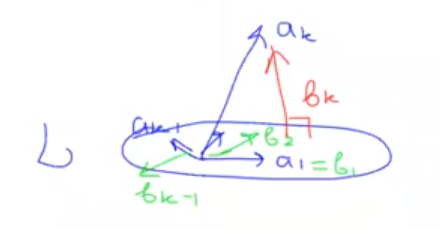
\includegraphics[width=\textwidth]{pic04}
		\end{minipage}
		\begin{minipage}{0.7\textwidth}
			$b_k = a_k - \underbrace{\sum\limits_{i=1}^{k-1} c_i b_i}_{y\in L} \; \; \; 
			\begin{matrix}
				a_k = y + b_k \leftarrow \text{ортогон. составляющая } a_k \\
				\text{ относительно } L\\
				\underset{i = 1\ldots k-1}{b_k \perp n_i} \Rightarrow \boxed{b_k \perp L}
			\end{matrix}$
		\end{minipage}
	\end{remark}
\end{document}